% ledger.tex -- Results 4.4: what the twin predicted. 17 Oct (v3_full): skel_ledger merged; T13 generated
% (tools/thesis_freeze_tables.py, docs/analysis/thesis_tables_T10_T13_2026-10-16.md; W4 twin column n = 1 on the freeze
% tree, must not say "W4 n = 3"); the parity figure moved here from 4.1; the 1 m carry bands (card
% docs/experiments/2026-10-16_bands_1m.md, rule signed 17 Oct, bands frozen ~19:54, tools/n2_bands.py); the pattern
% paragraph from the inventory's F4 and the counter-swing analysis (docs/analysis/counter_swing_2026-10-12.md).
% The band rule and the frozen 14 Oct bands are the signed
% freeze (docs/freeze_2026-10-14.md sections 1.4 and 2.4, Wesley 11 Oct 17:24 and 17:35; code tools/release_bands.py).
% The ledger's rows come after each rig day. No run ids: the twin sets are given by count and value.

\subsection{The prediction ledger}
\label{sec:ledger}

From 14 October on, each rig cell is to be predicted by the rig twin under a band frozen before it flies, and scored
afterwards. The rule was signed on 11 October, before the first flight it applies to, so no band is chosen by its
outcome. No rig row is scored yet: the cells with bands have not flown, and the attach flights of 14--15 October have no
band, since the twin's magnet catches at the instant of contact. The ledger is so far a protocol.

\paragraph{The band.} For a rig cell the twin flies the same configuration on the same code tree, before the
rig does, and gives a set of tilt rises $\{\Delta\theta_{\mathrm{twin}}\}$ (Section~\ref{sec:metrics}; cut at
$t_e+15$\,s, the shortest hold the rig flies). The band is
\begin{equation}
  \Big[\,\max\big(0,\ \min\Delta\theta_{\mathrm{twin}}\,f_{\mathrm{lo}}-2\sigma_{\mathrm{rig}}\big),\quad
  \max\Delta\theta_{\mathrm{twin}}\,f_{\mathrm{hi}}+2\sigma_{\mathrm{rig}}\,\Big].
  \label{eq:band}
\end{equation}
The class factors come from the four 8 October rig flights and their twin pairs, each pair cut at the rig
flight's own event-to-LAND: for each pair the ratio $\rho$ of the rig's $\Delta\theta$ to the twin pair's
mean, and within a class, announced or unannounced releases, $f_{\mathrm{lo}}=\min\rho$ and
$f_{\mathrm{hi}}=\max\rho$; a class with fewer than two pairs takes $f_{\mathrm{lo}}=f_{\mathrm{hi}}=1$.
$\sigma_{\mathrm{rig}}$ is the pooled $\sigma_{\mathrm{pre}}$ of the four 8 October rig pre-windows, the
ring's own rocking in hover. The factors are assumed to carry the rig-to-twin gap across one change of
configuration: the 8 October pairs flew the reference integral, and the 14 October flights fly the model
integral with the freed UAV disarmed alone.

\paragraph{Scoring.} Only rows whose band was frozen before the flight are scored; the 8 October pairs appear
as agreement, not as predictions. Each scored flight gets three readings: a hit or a miss; the band's width;
and $\ln(\Delta\theta_{\mathrm{rig}}/\Delta\theta_{\mathrm{mid}})$, where the twin midpoint is the mean of the
twin set's smallest and largest values. Two naive predictors are scored the same way, as bands of the same
$\pm2\sigma_{\mathrm{rig}}$: ``the rig equals the twin'',
$[\min\Delta\theta_{\mathrm{twin}}-2\sigma_{\mathrm{rig}},\ \max\Delta\theta_{\mathrm{twin}}+2\sigma_{\mathrm{rig}}]$,
and ``the rig equals its previous flight of the same cell'', which for the 14 October hover and circle releases
are the 8 October unannounced hover and circle flights, differing in the integral mode and in how the freed
UAV lands. A twin arm clears a rig fix only if the twin reproduced the failure.

\paragraph{The bands for the release cells.} Frozen on 11 October from twin runs on the code tree then planned for
14 October, released at the twin's timing: the hover release 6--7\,s after the ring reaches 1.0\,m, the circle release about 10\,s
into the circle (Table~\ref{tab:ledger_bands}). Neither release flew on 14 or 15 October, whose flights were the attach
(Section~\ref{sec:res_join}), so no ledger row is scored yet; on the freeze code tree the twin's own runs of both cells
lie inside their bands (Table~\ref{tab:T13}), which says the bands still stand on the current code, not that they
predict the rig.

\begin{table}[h]
\centering
\small
\caption{The frozen bands for the hover and circle releases: unannounced, the freed UAV disarmed alone, the model
integral. Factors from the three unannounced 8 October pairs (rig-to-twin ratios 0.85, 1.05 and 1.70); the one
announced pair (1.71) leaves its class at $f=1$.}
\label{tab:ledger_bands}
\begin{tabularx}{\textwidth}{>{\raggedright\arraybackslash}Xccccc}
\toprule
Flight & Twin $\Delta\theta$ ($^\circ$) & Midpoint & $f_{\mathrm{lo}}$, $f_{\mathrm{hi}}$ & $\sigma_{\mathrm{rig}}$ ($^\circ$) & Band ($^\circ$) \\
\midrule
Hover release & 6.12, 5.74, 6.67 (3 runs) & 6.21 & 0.851, 1.704 & 1.568 & [1.75, 14.51] \\
Circle release & 4.87, 5.91 (2 runs) & 5.39 & 0.851, 1.704 & 1.568 & [1.00, 13.20] \\
\bottomrule
\end{tabularx}
\end{table}

The bands are wide by construction: the rig-to-twin ratios span a factor of two and $2\sigma_{\mathrm{rig}}$
adds about $3^\circ$, so a hit alone says little and the three readings carry the claim. In the circle twin
the three-UAV ring settles to a steady tilt of about 2.7$^\circ$ after the release and is back in its band only
after 13.5--14.0\,s, so its $\Delta\theta$ is set by the new steady tilt more than by the release itself, unlike
the 8 October circle pair; the circle flight is read with that in mind.

% generated by tools/thesis_freeze_tables.py; run ids in docs/figures/PROVENANCE.md
\begin{table}[htbp]
  \centering
  \footnotesize
  \caption[The twin against the rig]{The twin against the rig (T13), on the tilt rise $\Delta\theta$. Upper rows,
  scored once flown: the hover and circle releases of the ledger, the twin on the freeze code tree (the hover one run
  at the band's own timing) against the bands of Table~\ref{tab:ledger_bands}. Lower rows, agreement only: the four
  8 October flights against the twin flying the same configuration (the reference integral, the freed UAV landing with
  the fleet), both cut at the rig flight's hold; factor: the rig's $\Delta\theta$ over the twin pair's mean. Rate fix:
  before or after the rig's body rates were sent at full precision.}
  \label{tab:T13}
  \begin{tabularx}{\textwidth}{>{\raggedright\arraybackslash}Xcccccc}
    \toprule
    Cell & Twin $\Delta\theta$ ($^\circ$), $n$ & Rig $\Delta\theta$ ($^\circ$), $n$ & Factor & Rate fix & Band ($^\circ$) & Scored \\
    \midrule
    Hover, unannounced & 6.0, 1 & not yet flown & -- & after & 1.75--14.51 & when flown \\
    Circle, unannounced & 6.7--7.1, 2 & not yet flown & -- & after & 1.00--13.20 & when flown \\
    \midrule
    \multicolumn{7}{l}{\emph{8 October pairs (agreement, not scored)}} \\
    Hover, announced & 6.0--7.1, 2 & 11.2, 1 & 1.71 & before & -- & no \\
    Hover, unannounced & 6.0--6.4, 2 & 5.3, 1 & 0.85 & before & -- & no \\
    Hover, unannounced, 150$^\circ$ gap & 14.6--17.4, 2 & 16.9, 1 & 1.05 & before & -- & no \\
    Circle, unannounced & 4.0--5.4, 2 & 8.0, 1 & 1.70 & before & -- & no \\
    \bottomrule
  \end{tabularx}
\end{table}


\paragraph{Agreement before the rule.} The four releases of 8 October predate the rule and are agreement only
(Table~\ref{tab:T13}, lower rows; Figure~\ref{fig:twin_rig_parity}). The twin flying the same configuration matched
the tilt rise of the unannounced hover and 150$^\circ$-gap releases within a quarter (0.85 and 1.05 times the twin)
and how soon the planner finds a loss to within 0.1\,s, but the announced hover release and the circle release rose
1.7 times the twin, the rig's ring dipped up to 2.5 times as far, and before the release it sat 1.9--3.1 times as far
from its reference.

\begin{figure}[htbp]
\centering
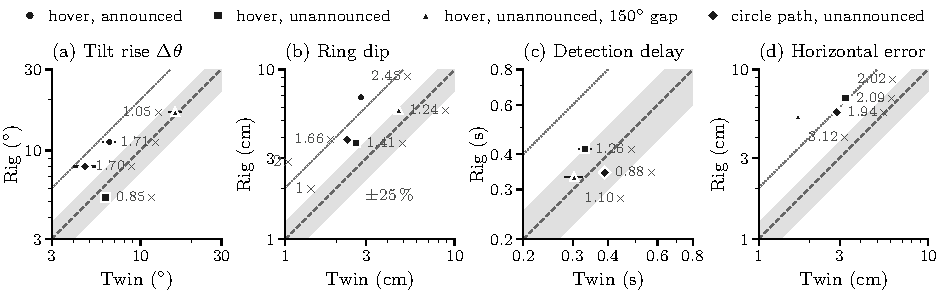
\includegraphics[width=\textwidth]{Images/twin_rig_parity.pdf}
\caption[The twin against the rig]{The rig against its twin for the four releases of 8 October (four UAVs,
0.86\,kg ring at 1.0\,m; one marker per flight; 150$^\circ$ gap: the three left on the ring leave a 150$^\circ$ gap
between two of them), each metric computed the same way from both, on logarithmic axes: $x$, the twin flying the same
configuration (mean of two runs; bar: their range, hidden where it is shorter than the marker); $y$, the rig (one run).
Dashed: $y = x$; grey band: within 25\,\% of the twin; dotted: the rig twice the twin. (a) Tilt rise $\Delta\theta$:
the peak of the ring's tilt-vector departure from its mean over the 5\,s before the release, from the release to the
rig flight's LAND, the twin cut at the same hold. (b) Ring dip: its lowest height error in the 3\,s after the release.
(c) Detection delay: from the release to the planner finding an unannounced release (an announced release needs
none). (d) Horizontal error: the ring's mean distance from its reference over the 10\,s before the release. Within
25\,\% of the twin: the tilt rise of the unannounced hover and 150$^\circ$-gap releases (0.85 and 1.05 times the twin),
the dip of the 150$^\circ$-gap release, and two of the three detection delays (the third is 1.26 times the twin; all
three within 0.1\,s). The announced hover release and the circle release rose 1.7 times the twin; the other three dips
were 1.4--2.5 times the twin's, and the horizontal error was 1.9--3.1 times (5.3--6.8\,cm against 1.7--3.3\,cm).}
\label{fig:twin_rig_parity}
\end{figure}

\paragraph{The carry bands for the next rig day.} The next rig day flies the carriers on 1\,m cables, so the carry
cells were given bands on the 1\,m worlds before it, under a rule signed on 17 October: the band is
$[\max(0, \min - 2\sigma_{\mathrm{rig}}), \max + 2\sigma_{\mathrm{rig}}]$ on the path RMSE and on the peak tilt, from
the path's start to LAND, over three twin runs per cell, with no class factor since no rig carry pair exists on the
current controller, and $\sigma_{\mathrm{rig}}$ from the rig's three-carrier steady hover of 14 October (10.3\,mm on the
path error, 1.50$^\circ$ on the tilt). Because $2\sigma_{\mathrm{rig}}$ is larger than the twin's spread, each band
tests its upper side only: a rig flight misses when its path RMSE exceeds about 30--46\,mm or its peak tilt about
4.6--9.2$^\circ$, depending on the cell (Appendix~\ref{sec:app_bands}).

\paragraph{The pattern so far.} Where the twin and the rig have been compared, on the 8 October releases that
predate the bands, the twin matched the reactive release and missed what it does not model. It has no magnet holding limit: on the layout and pull of L2 its ring peaked at
5.5$^\circ$ (one run) where the rig's capsized. It has no counter-swing: on the rig the survivors' thrust
swung against the step when the plan arrived, in 9 of 9 survivors of the three unannounced 8 October releases
(0.14--1.40\,N at about 1\,Hz). Its ring sits closer
to its reference before a release (1.7--3.3 against 5.3--6.8\,cm). And its rigid rods behave where the rig's tethers
would go slack: the newcomer tipped on 12 of 48 landings after a fold-in in the twin, which the rig's tether should
not do.

\pendingfig{fig:F16}{The ledger: for each rig flight, the band frozen before it (bar) and the rig value (dot), with the
naive predictors.}{the hover and circle releases (L8, L9) and the 1\,m carry cells, from the next rig day}
